\lstinputlisting[language=bash,basicstyle=\small]{python_codes/fieldstone_63/keywords}

{\sl This stone was developed in collaboration with Taka Shinohara}.
\index{contributors}{Taka Shinohara}

This stone aims at replicating the findings of Wong and Wu (1995) \cite{wowu95}.

\begin{center}
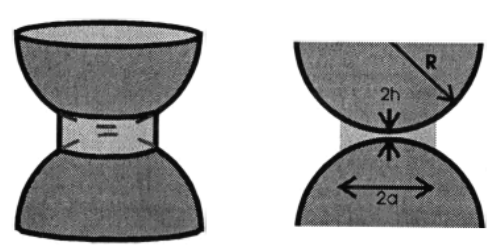
\includegraphics[width=8cm]{python_codes/fieldstone_63/images/yoyo}
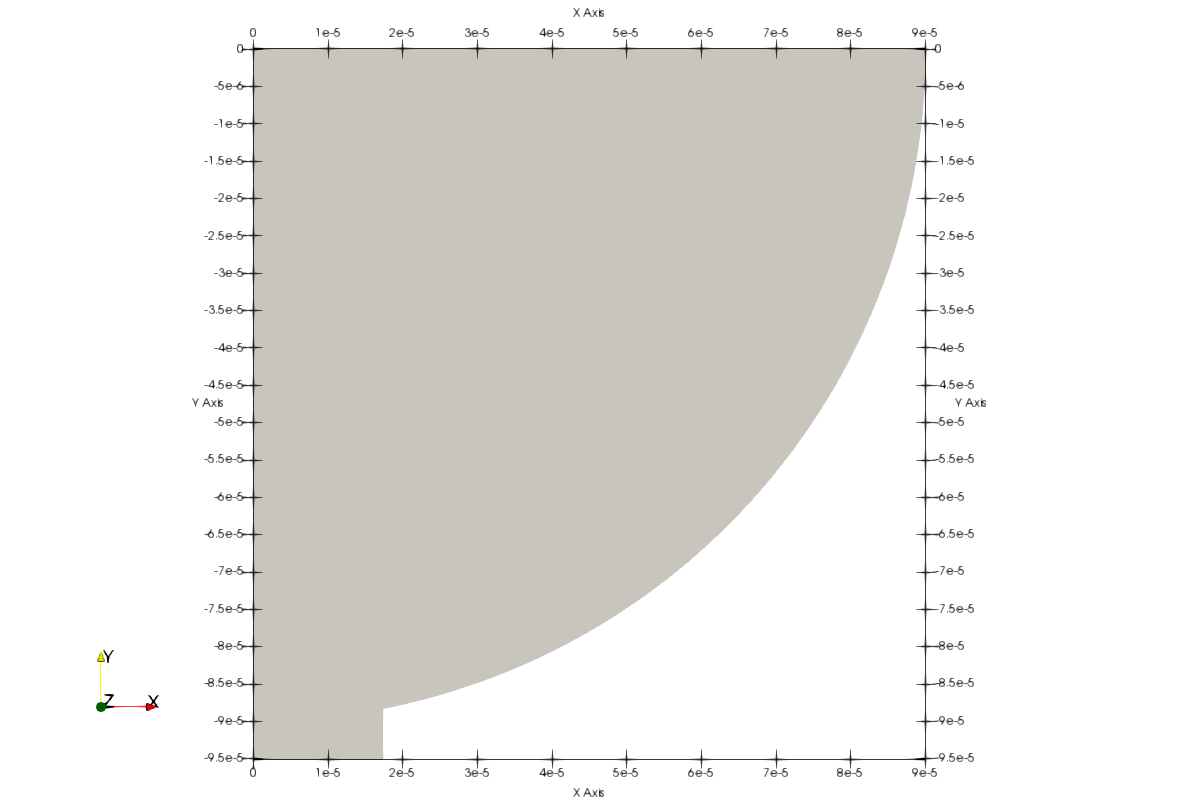
\includegraphics[width=6cm]{python_codes/fieldstone_63/images/domain}\\
{\captionfont Left: model of cemented granular system for 
axisymmetric finite element analysis (taken from \cite{wowu95}); Right: 
Domain for a\_fac=0.2 and h\_fac=5/90 and $R=90\mu m$.}
\end{center}

Wong \& Wu use a quadtree-based mesh as shown hereunder while we 
use triangles:

\begin{center}
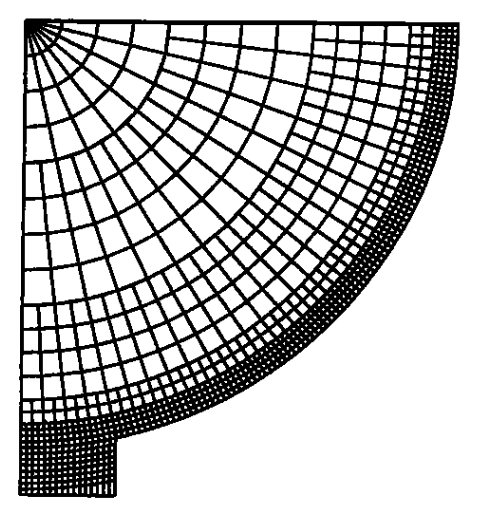
\includegraphics[width=5.5cm]{python_codes/fieldstone_63/images/wowu95b}
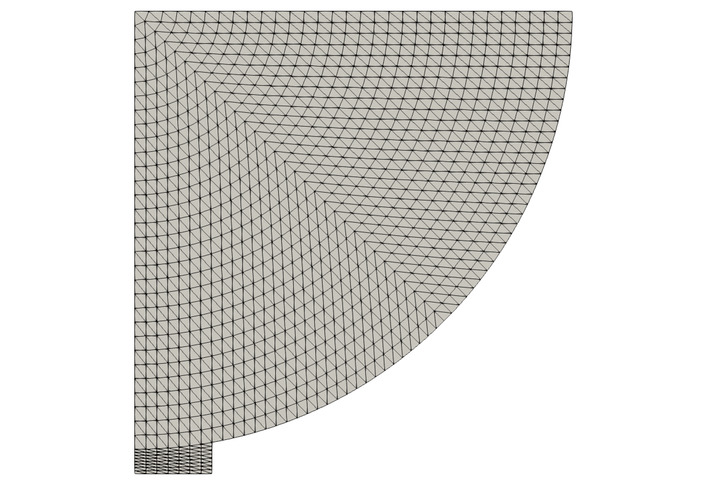
\includegraphics[width=8cm]{python_codes/fieldstone_63/images/mesh}\\
{\captionfont Left: mesh used in \cite{wowu95}; 
Right: low resolution fieldstone mesh.}
\end{center}


\begin{center}
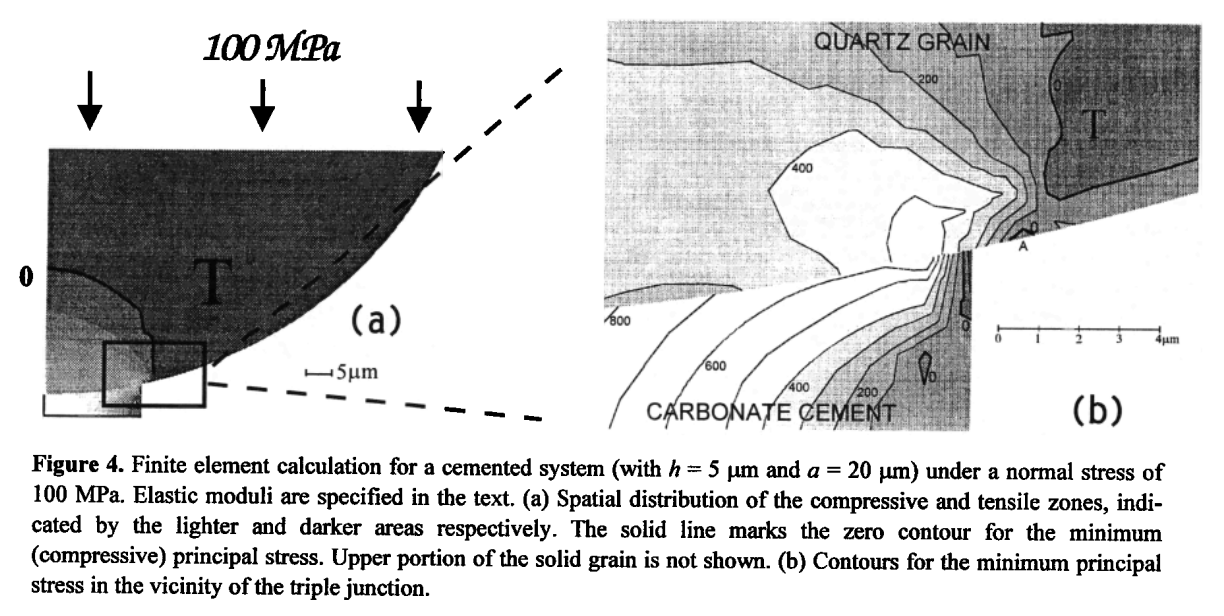
\includegraphics[width=12cm]{python_codes/fieldstone_63/images/wowu95}\\
{\captionfont Taken from \cite{wowu95}}
\end{center}

Write about:

- material properties

- how the mesh is built

- boundary conditions (traction b.c. are described in Section~\ref{ss:openbc})

- principal stresses are computed as explained in Section~\ref{sec:princ_stress}.

- 7-point integration for elemental averages

- gravity plays no role

- projection of derivative quantities onto nodes

\begin{center}
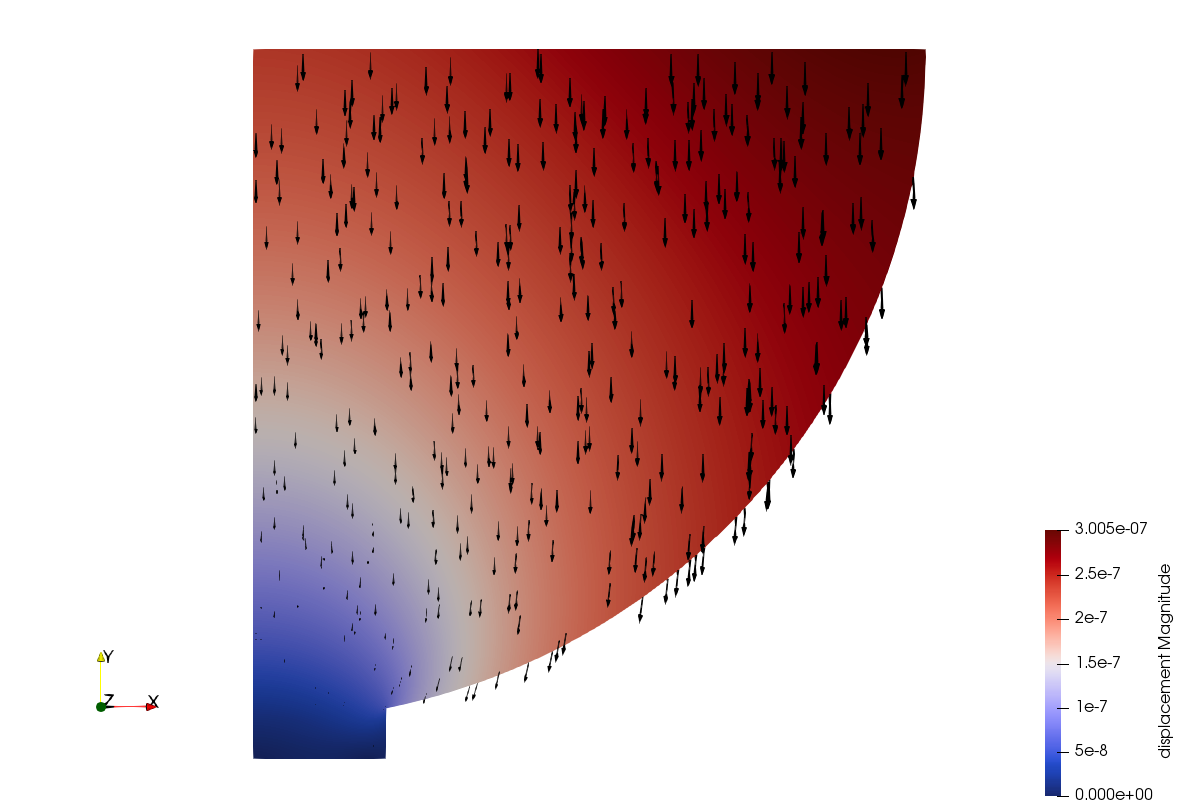
\includegraphics[width=5cm]{python_codes/fieldstone_63/results/disp}
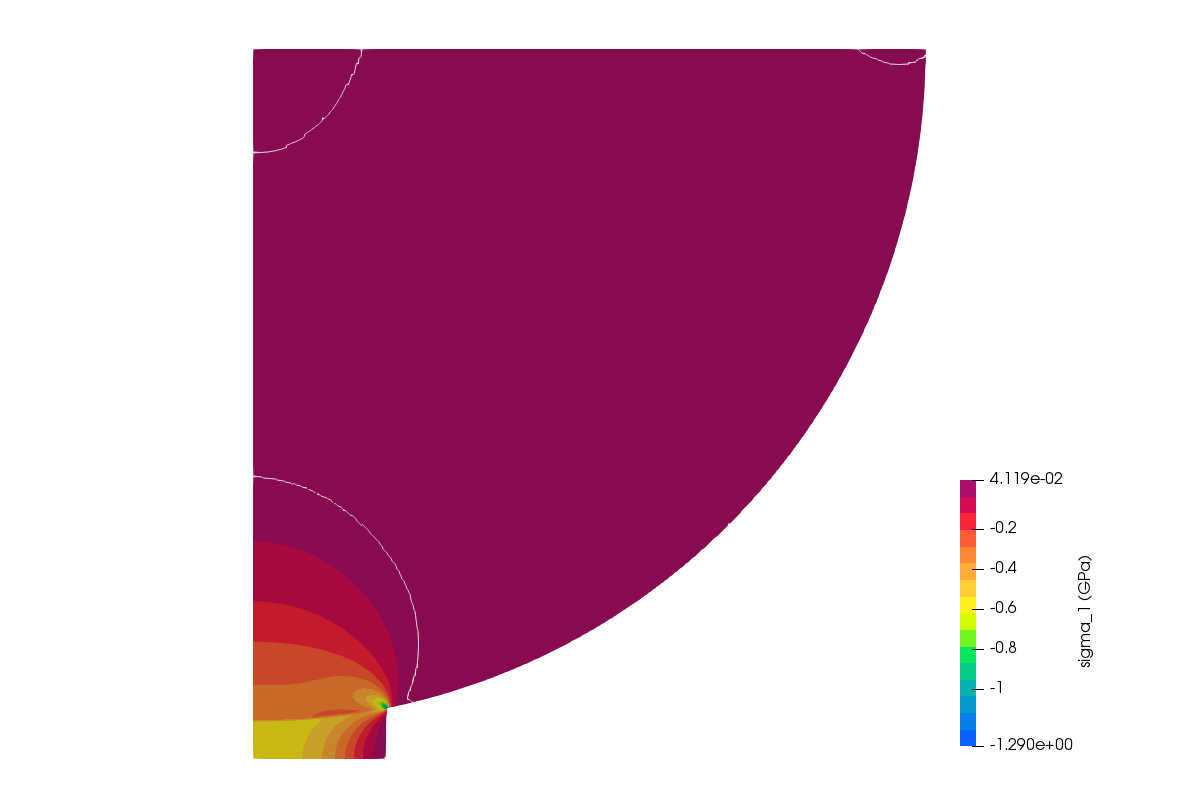
\includegraphics[width=5cm]{python_codes/fieldstone_63/results/sigma1}
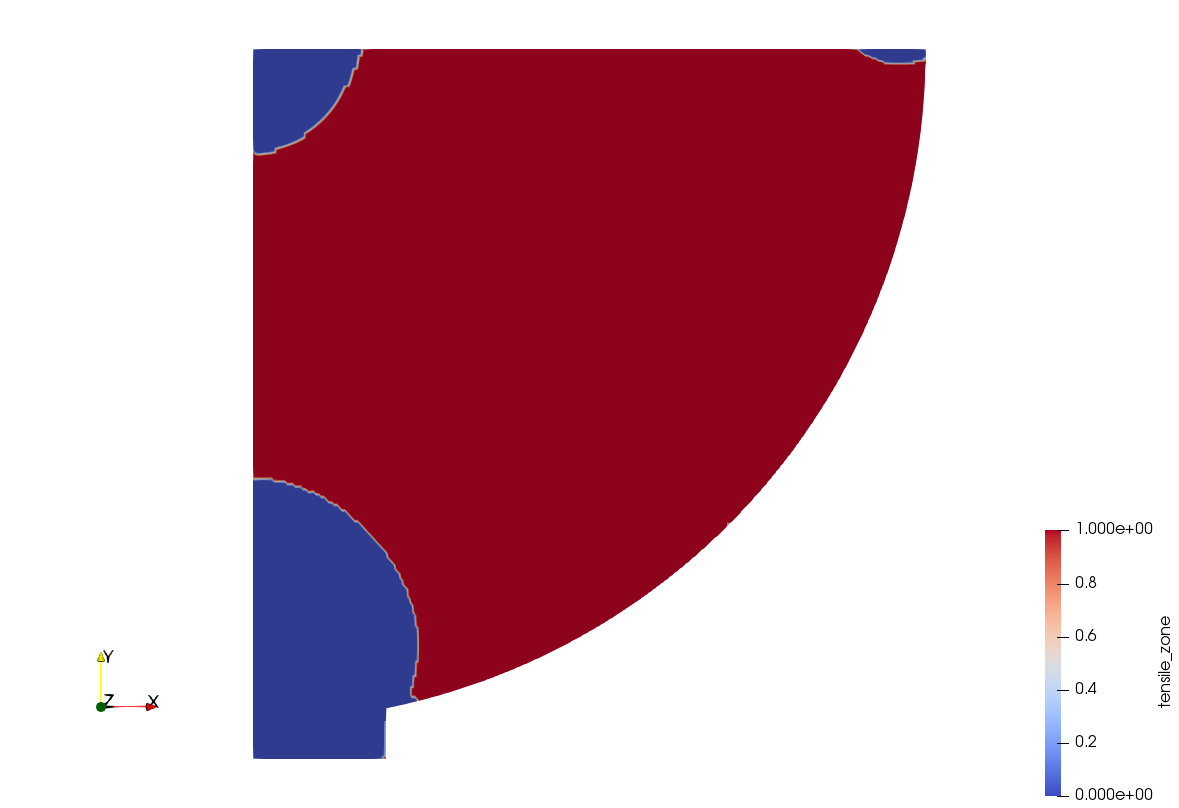
\includegraphics[width=5cm]{python_codes/fieldstone_63/results/tensilezone}\\
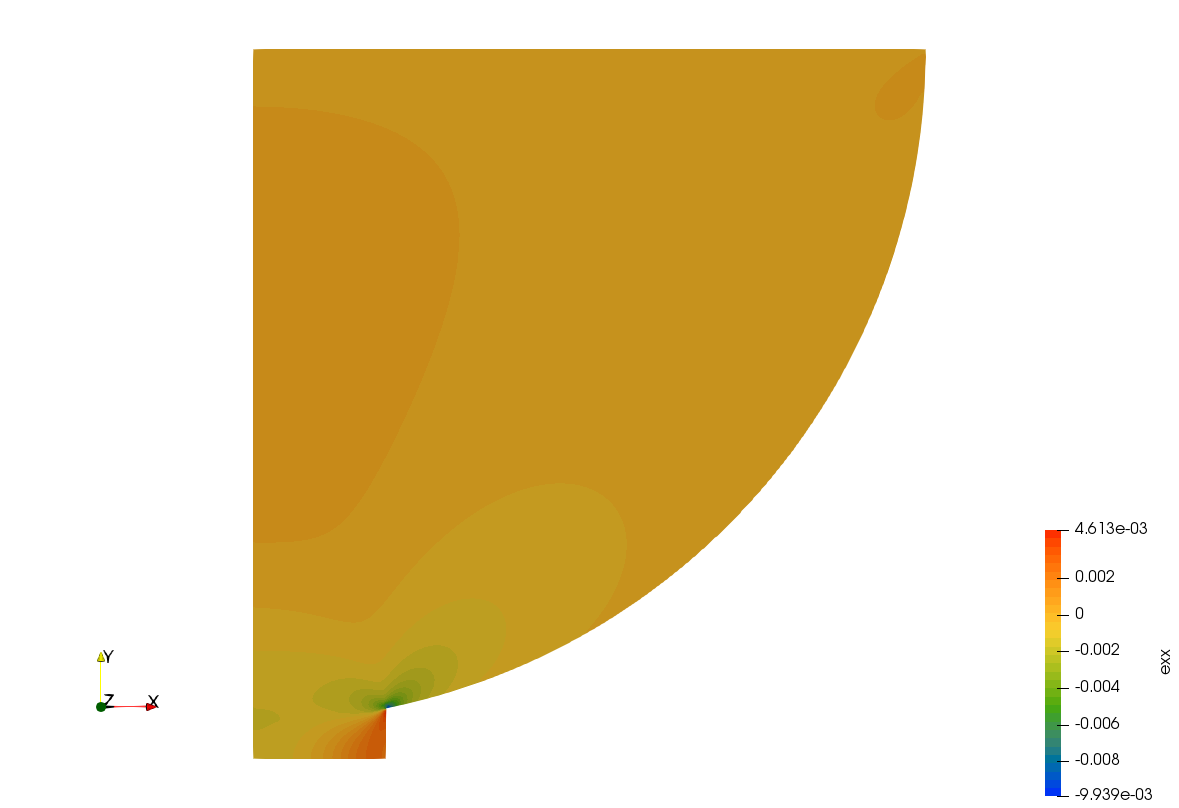
\includegraphics[width=5cm]{python_codes/fieldstone_63/results/exx}
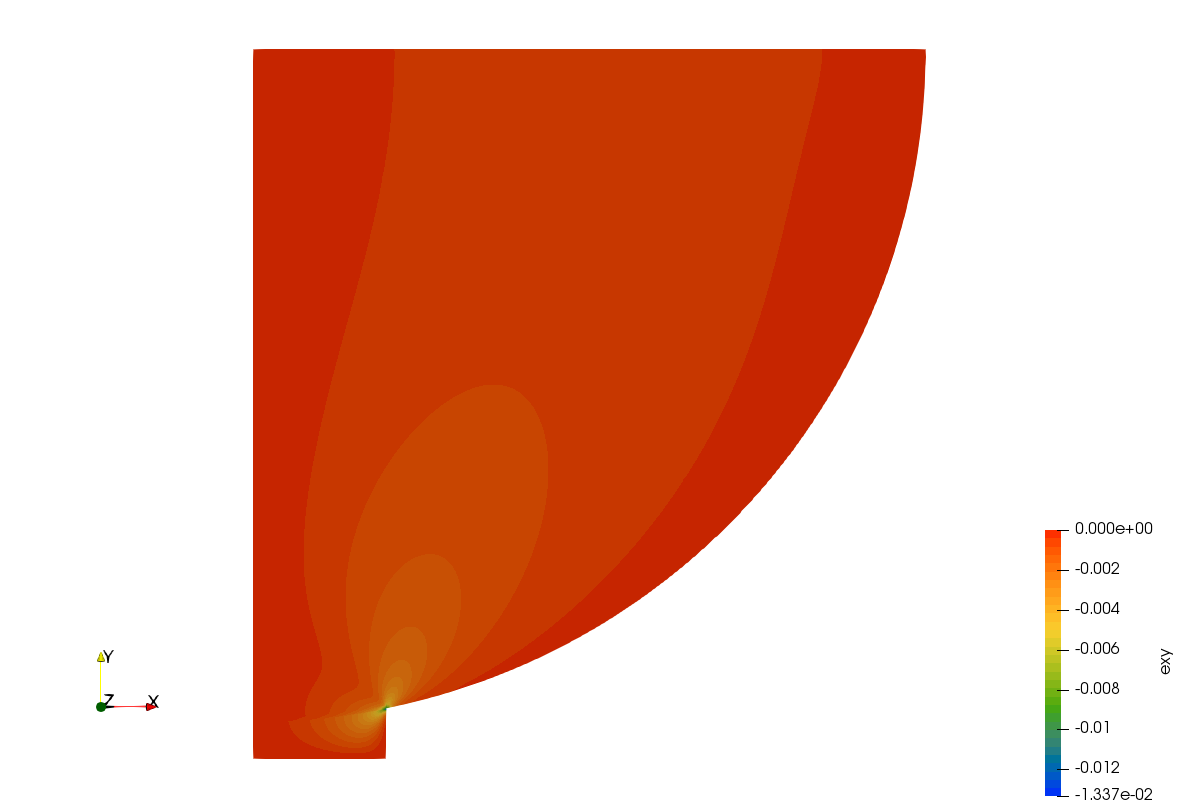
\includegraphics[width=5cm]{python_codes/fieldstone_63/results/exy}
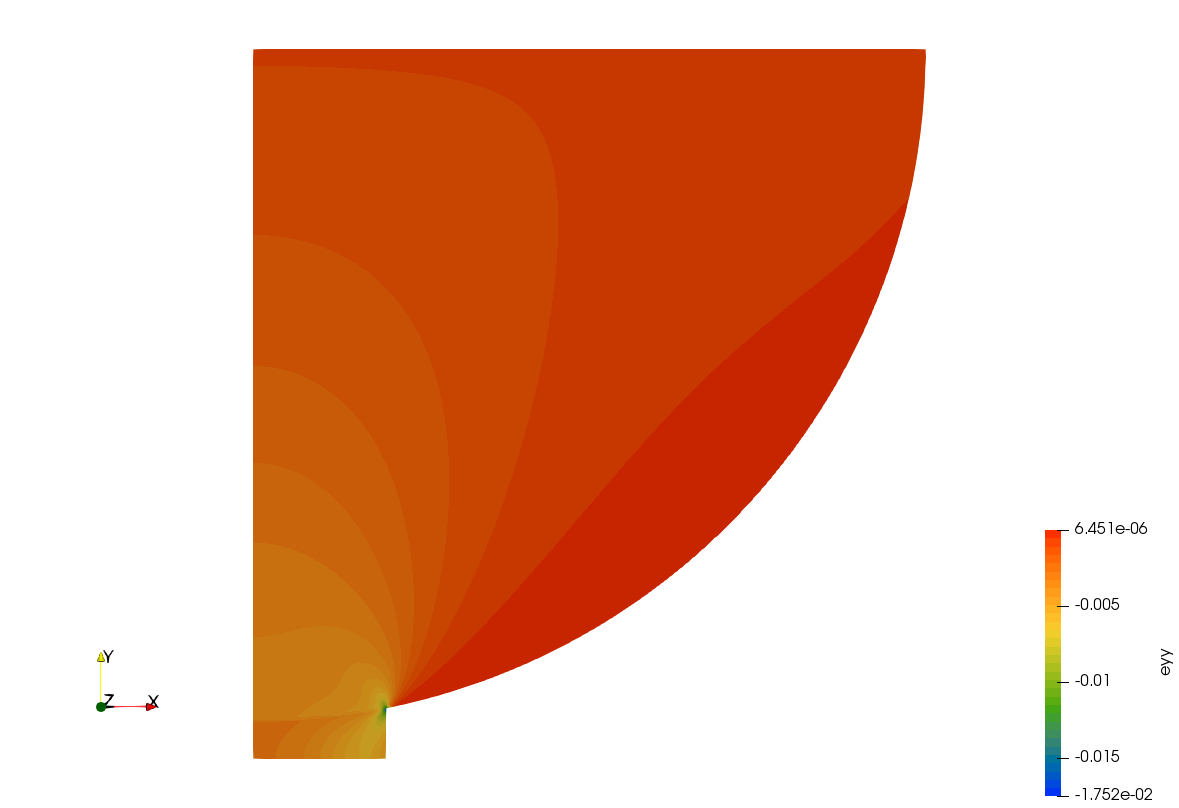
\includegraphics[width=5cm]{python_codes/fieldstone_63/results/eyy}\\
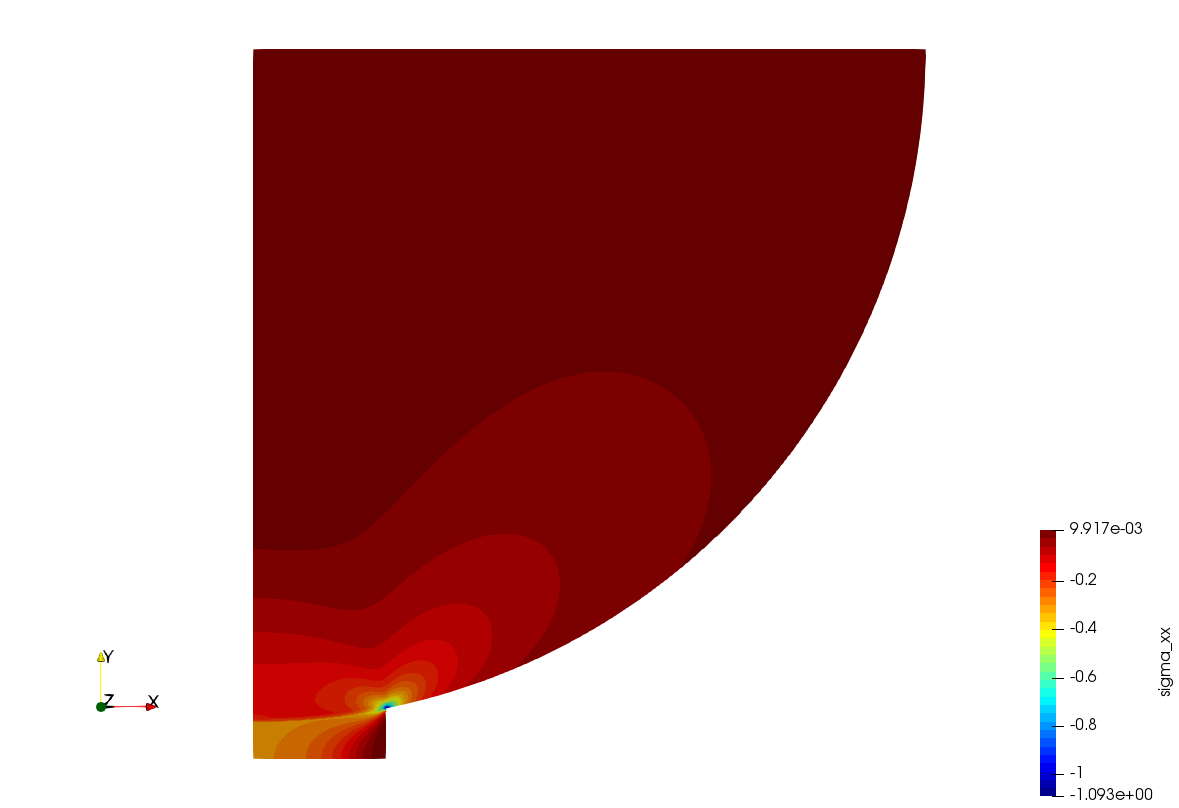
\includegraphics[width=5cm]{python_codes/fieldstone_63/results/sigmaxx}
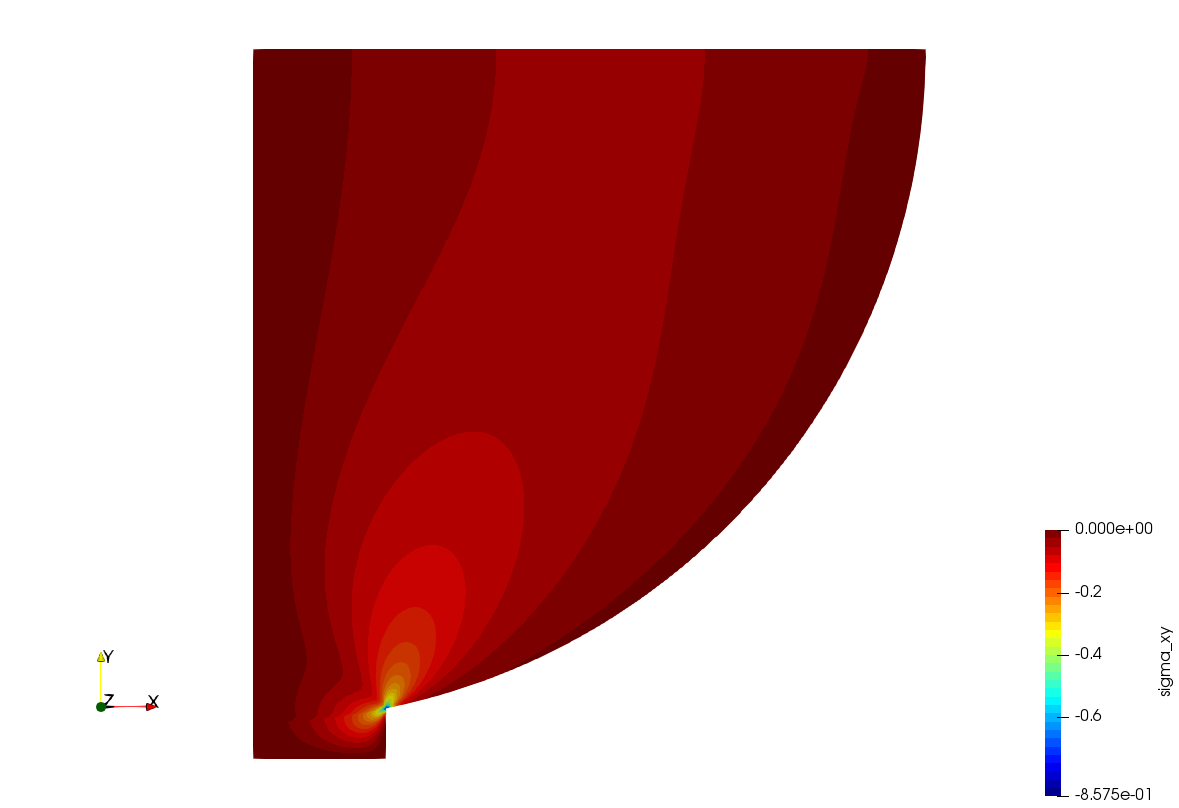
\includegraphics[width=5cm]{python_codes/fieldstone_63/results/sigmaxy}
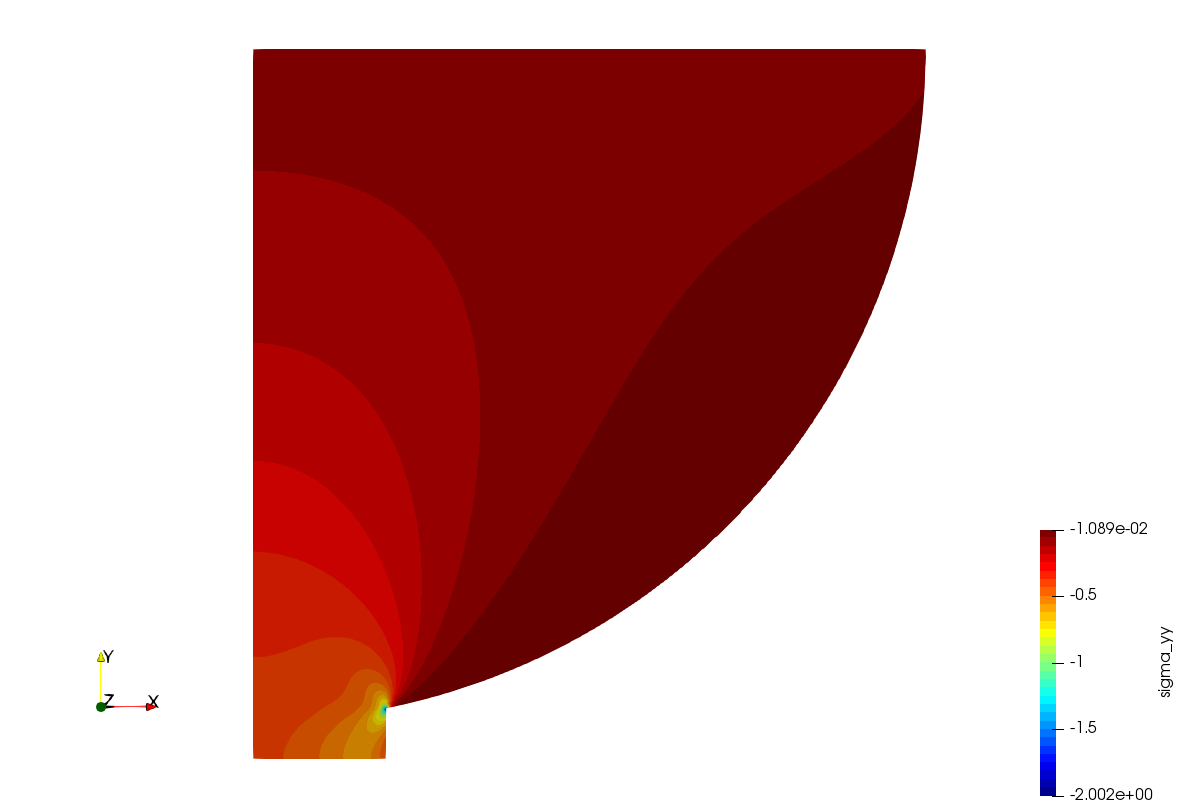
\includegraphics[width=5cm]{python_codes/fieldstone_63/results/sigmayy}
\end{center}

